\documentclass{yqart}

%%%%%%%%%% Additional Settings %%%%%%%%%%
\usepackage{kantlipsum}                 %
                                        %
%%%%%%%%%%%%%%%%%%%%%%%%%%%%%%%%%%%%%%%%%

%%%%%%%%%%%% Title Settings %%%%%%%%%%%%%                                        
\title{Your Title}                      %
\subtitle{An optional subtitle}         %
\author{First Author}                   %
\email{first@author.com}                %
\website{https://first.com/}            %
\author{Second Author}                  %
\email{second@author.com}               %
\affiliation{First Institution}         %
\author{Third Author}                   %
\email{third@author.com}                %
\affiliation{Second Institution}        %
\date{20 October 2023}                  %
%%%%%%%%%%%%%%%%%%%%%%%%%%%%%%%%%%%%%%%%%

\begin{document}

\maketitle

%%%%%%%%%%%%%%% Abstract %%%%%%%%%%%%%%%%
% abstracts are optional                %
\begin{abstract}                        %
    An optional abstract. \kant[1]      %
\end{abstract}                          %
%%%%%%%%%%%%%%%%%%%%%%%%%%%%%%%%%%%%%%%%%

%%%%%%%%%%%%%% Keywords %%%%%%%%%%%%%%%%%
% keywords are optional                 %
\keywords{your, optional, keywords}     %
%%%%%%%%%%%%%%%%%%%%%%%%%%%%%%%%%%%%%%%%%



\section{Sections}\label{sec:sections}

An example section. Use \verb|\autoref| to refer to labels. For example, \autoref{sec:sections} is a section, \autoref{subsec:subsections} is a sub-section. Use \verb|\cite| to write citations \cite{some:article}.

\subsection{Subsections}\label{subsec:subsections}
An example subsection.

\subsubsection{Subsubsections}
An example subsubsection

\paragraph{Paragraphs}
An example paragraph

\section{Math}
An example equation is shown in \autoref{eq:Ps}.

\begin{equation}\label{eq:Ps}
    \mathbb{P}(S)=\{T \in \mathcal{G} ~|~ S = T \lor \textbf{Path}_\mathcal{G}(S,T), T \text{ non-abstract}\}
\end{equation}

Alternatively you can write math like $f(x)=x+1$ or \[y=mx+c\]

\subsection{Theorem Environments}

\begin{definition}\label{defn:P}
    We let $\mathbb{P}(S)$ be the following.\[\mathbb{P}(S)=\{T \in \mathcal{G} ~|~ S = T \lor \textbf{Path}_\mathcal{G}(S,T), T \text{ non-abstract}\}\]
\end{definition}

\begin{remark}\label{remark:P}
    \autoref{defn:P} is useless since it has already been defined by \autoref{eq:Ps}. Well, so is \autoref{remark:P}.
\end{remark}

\begin{example}
    This is an example.
\end{example}

\begin{lemma}\label{lemma:blue}
    The colour blue exists.
\end{lemma}

\begin{proposition}\label{prop:sky}
The sky is blue.
\end{proposition}
\begin{proof}
    Use your eyes and see \autoref{fig:duck}.
\end{proof}
\autoref{lemma:blue} and \autoref{prop:sky} give us \autoref{thm:ocean}.
\begin{theorem}\label{thm:ocean}
    The ocean is blue
\end{theorem}
\begin{proof}
    Use your eyes
\end{proof}
\begin{corollary}
    Fish swim.
\end{corollary}
\begin{proof}
    \begin{prooftree}
        \hypo{\Gamma, x:\texttt{T} \vdash e: \texttt{U}}
        \infer1[\scriptsize\scshape Abs]{\Gamma \vdash \lambda x.e : \texttt{T} \rightarrow \texttt{U}}
    \end{prooftree}
\end{proof}
\begin{conjecture}
    Some fish can fly.
\end{conjecture}

\section{Graphics}
\autoref{fig:duck} shows a duck. \autoref{tab:sometable} shows a table consisting of some data. Finally, \autoref{alg:analg} shows an algorithm for saying hello to everyone. Source code for \autoref{alg:analg} is shown in \autoref{lst:helloworld}.

\begin{figure}[ht]
\centering
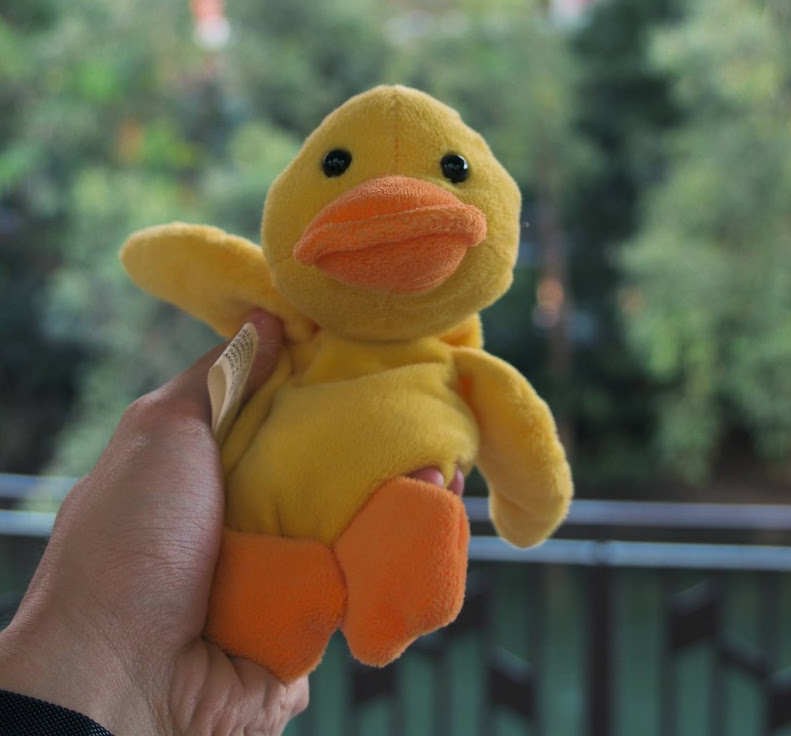
\includegraphics[width=5cm]{duck.jpg}
\caption{A duck.}\label{fig:duck}
\end{figure}

\begin{table}[ht]
    \centering
        \caption{A table}
    \label{tab:sometable}

    \begin{tabular}{lcccccl}\toprule
    & \multicolumn{3}{c}{$a=b$} & \multicolumn{3}{c}{$c=d$}
    \\\cmidrule(lr){2-4}\cmidrule(lr){5-7}
               & $mv$  & Rel.~err & Time    & $mv$  & Rel.~err & Time\\\midrule
    \texttt{BenchA}    & 11034 & 1.3e-7 & 3.9 & 15846 & 2.7e-11 & 5.6 \\
    \texttt{BenchB} & 21952 & 1.3e-7 & 6.2 & 31516 & 2.7e-11 & 8.8 \\
    \texttt{BenchC} & 15883 & 5.2e-8 & 7.1 & 32023 & 1.1e-11 & 1.4e1\\
    \texttt{BenchD}   & 11180 & 8.0e-9 & 4.3 & 17348 & 1.5e-11 & 6.6 \\\bottomrule
    \end{tabular}
\end{table}

\begin{algorithm}[ht]
\caption{Saying Hello}\label{alg:analg}
\begin{algorithmic}[1]
\Statex \textbf{Input}: A list of names
\Statex \textbf{Output}: Says hello to everyone in the console
\Function{HelloWorld}{\textit{names}}
    \ForEach{$n\in\textit{names}$}
        \State $y\gets \texttt{`Hello '} ~||~ x$ \Comment{$||$ represents concatenation}
        \State $\textit{print}(y)$
    \EndFor
    \State \Return 1
\EndFunction

\end{algorithmic}
\end{algorithm}

\begin{lstlisting}[language=scala, label={lst:helloworld}, caption={A Scala program for saying hello to everyone}, float]
def helloWorld(names: Seq[String]): Int =
    names.map("Hello " + _)
         .foreach(println)
\end{lstlisting}

More details are described in \autoref{app:first} and \autoref{app:second}.

\section{Conclusion}
\kant[2]

%Bibliography
\bibliographystyle{alpha}  
\bibliography{references}  

\appendix

\section{An Appendix}\label{app:first}
Have you removed your appendix?

\subsection{Part of the appendix}
\kant[3]

\section{Another Appendix}\label{app:second}
\kant[4-6]

\end{document}
